\section{Signale im Zeitbereich}
  \subsection{Signalcharakterisierung}
  \begin{itemize}
      \item{\textbf{Kontinuierlich \hfill $\longleftrightarrow$ \hfill Diskret}}
      \item{\textbf{Deterministisch \hfill $\longleftrightarrow$ \hfill Stochastisch}}\\
          Deterministisch: $x(t)$ mathematisch beschreibbar.
          Stochastisch: Signal zufällig, kein $x(t)$.
      \item{\textbf{Periodisch \hfill $\longleftrightarrow$ \hfill Aperiodisch}}\\
              Periodisch, wenn $x(t)=x(k \cdot t+T_p)$ mit
			  $T_p = \frac{2\pi}{k}$ \\
              $T_p$: Grundperiode/Periodendauer
      \item{\textbf{Gerade $x(-t)=x(t)$ $\leftrightarrow$ Ungerade: $x(-t)=-x(t)$}}\\
          \begin{mdframed}[style=exercise,frametitle=Zerlegung des Signals:]
              - gerader Anteil: \quad $x_G=\frac{1}{2}\left[x(t)+x(-t)\right]$\\
              - ungerader Anteil: \quad $x_U=\frac{1}{2}\left[ x(t)-x(-t) \right]$\\
              - gemischtes Signal: $x(t)=x_G + x_U$
          \end{mdframed}
          \begin{center}
              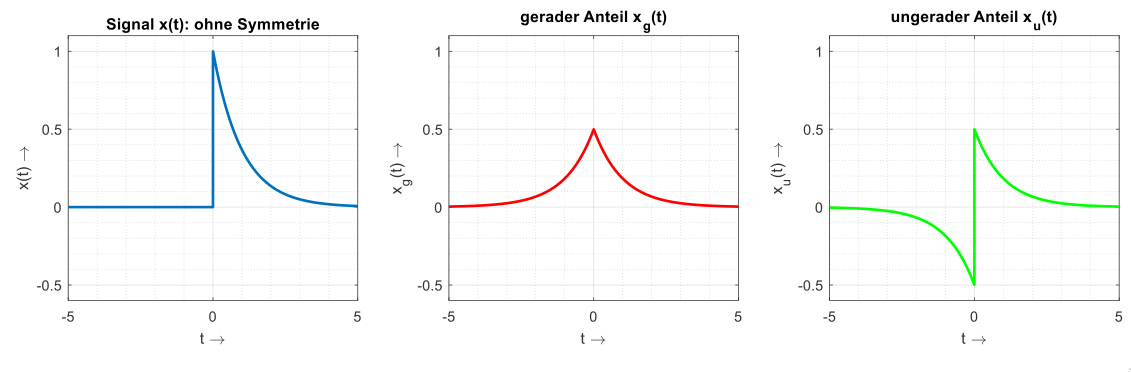
\includegraphics[width=0.43\textwidth]{Signale/gerade_ungerade_signal}
          \end{center}
      \item{\textbf{Energie \hfill $\longleftrightarrow$ \hfill Leistung}}\\
              (Gesamt-)Energie: \[E_x=\int_{t=-\infty}^{+\infty}\lvert x(t)\rvert^2 dt\ \quad (0<E_x<\infty)\]
              Mittlere Leistung: \[P_x=\lim_{T\to\infty}\frac{1}{2T}\int_{-T}^{+T}\lvert x(t)\rvert^2 dt \quad (0<P_x<\infty)\]
                {\small Ein Signal ist nie Energie- und Leistungssignal gleichzeitig!}
          
      \item{\textbf{Korrelationsfunktion}}\\
          {\small Ma{\ss} f\"ur die \"Ahnlichkeit
          zweier Energiesignale.}
              \[
                  r_{xy}(\tau) = \int_{-\infty}^{\infty}x(t)\cdot y(t+\tau) dt
              \]
      \item{\textbf{Signaloperationen}}\\
        {\small Manipulation/Transformation mit folgenden Parametern:}
            \[ \boxed{
				f(t) = A \cdot f(\pm b \cdot (t \mp t_0)) \leftrightarrow A \cdot f\left(\frac{t\mp t_0}{b}\right)
				}
			\]
		 \renewcommand{\labelitemii}{$\bullet$}
          \begin{itemize}
              \item{Zeitverschiebung $t-t_0$: nach \textbf{rechts}}!

              \item{Zeitskalierung:\\
              	Multiplikation mit $b>1$: Stauchung \\
              	Multiplikation mit $0<b<1$: Dehnung \\
              	Division durch $b>0$: Dehnung}

              \item{Zeitumkehr/-invertierung:\\ $-1 \cdot b$: Spiegelung an y-Achse}
              \item{Signalinvertierung:\\
              $-A\cdot f(t)$: Spiegelung an x-Achse}
              
          \end{itemize}
          \textbf{Wichtig}: Reihenfolge beachten!\\
          Erst Verschieben, dann Skalieren/Invertieren!
  \end{itemize}
  \subsection{Elementarsignale}
  \begin{mdframed}[style=exercise]
      \begin{itemize}[leftmargin=*]
          \item{Sprung-, Heavyside-Fkt., Einheitssprung $\varepsilon$, $\sigma$}
          \[ \varepsilon(t) = \varepsilon(k\cdot t) = 
             \begin{cases}
                 0 & \text{f\"ur } t < 0\\
                 1 & \text{f\"ur } t \geq 0
             \end{cases}
          \]
Verschoben, Start bei $t_0$:
        \[ \varepsilon(t-t_0) = 
          \begin{cases}
          	0 & \text{f\"ur } t_0 < 0\\
          	1 & \text{f\"ur } t_0 \geq 0
          \end{cases}
          \]
          \item{Dirac-Impuls $\delta$}
          \[
              \int_{t=-\infty}^{\infty} \delta(t) \, dt = 1
          \]
          \begin{itemize}
              \item Höhe = $\infty$, Fläche = 1.
              \item{Zusammenhang mit Sprungfunktion:}\\
                  $\boxed{\int_{\tau=-\infty}^{t}\delta(\tau)d\tau =
                  \varepsilon(t)}$
                  $\boxed{\dfrac{d}{dt}\varepsilon(t) =
                  \delta(t)}$
              \item{\textbf{Ausblend}eigenschaft}:
                  \[
                      \int_{-\infty}^{\infty}\delta(t-t_0)\cdot y(t) = y(t_0)
                  \]
              \item{Zeitskalierung: }
                  $\delta(at)=\dfrac{1}{\lvert a\rvert}\,\delta(t)$
          \end{itemize}
          \item{Dreieckimpuls $\Lambda$}
          Fläche = 1.
          \[ \Lambda(t) =
             \begin{cases}
                 0 & \text{f\"ur } \vert t\rvert > 1\\
                 1-|t| & \text{f\"ur } \vert t\rvert \leq 1
             \end{cases}
          \]
          \item{Rechteckfunktion $\operatorname{rect}$}\\
          $T:$ Breite
          \[ \hat{u} \cdot \operatorname{rect}\left(\frac{t}{T}\right) =
             \begin{cases}
                 \hat{u} & \text{f\"ur } \vert t\rvert \leq \frac{T}{2}\\
                 0 & \text{f\"ur } \vert t\rvert > \frac{T}{2}
             \end{cases}
          \]
          Darstellbar durch:\\ $1\cdot  \operatorname{rect}(t) = \varepsilon\cdot\left( t+\frac{1}{2} \right)-\varepsilon\cdot\left( t-\frac{1}{2} \right)$
          \item{Komplexe Exponentialfunktion}\\
          siehe Kap. \ref{ufkt}.
          \[ x(t)=\underline{A}\cdot e^{st} = \underline{A}\cdot e^{(\sigma+j\omega)t} = |\underline{A}|\cdot e^{j\varphi} \cdot e^{(\sigma+j\omega)t}
          \]
          \item Si-Funktion
                    \[ \operatorname{si}(x) =
          \begin{cases}
          	\dfrac{\sin(x)}{x} & \text{f\"ur } x\neq 0\\
          	1 & \text{f\"ur } x = 0
          \end{cases}
          \]
          Nullstellen: $\operatorname{si}(k\pi)=0$ für $k\ge1,\, k\in \mathbb{Z}$
      \end{itemize}
  \end{mdframed}
